\documentclass[a4paper,12pt]{article}
\usepackage{outline}
\usepackage{pmgraph}
\usepackage[normalem]{ulem}
\usepackage{comment} % enables the use of multi-line comments (\ifx \fi)
\usepackage{lipsum} %This package just generates Lorem Ipsum filler text.
\usepackage{fullpage} % changes the margin
\usepackage{listings}
\usepackage{color}
\usepackage{mdframed}
\usepackage{listings}
\usepackage{graphicx}
\graphicspath{ {../Screenshots/} }
\renewcommand{\lstlistingname}{Code Block}% Listing -> Algorithm
\renewcommand{\lstlistlistingname}{List of \lstlistingname s}% List of Listings -> List of Algorithms
%\title{\textbf{Lab 08: Introduction to Sequential Logic}
%\author{Joseph Martinsen \\ ECEN 248-510 \\ TA: Michael Bass}
\date{\today}

\linespread{1.5}
%--------------------Indention
\setlength{\parindent}{15pt}
\lstset{frame=shadowbox, rulesepcolor=\color{white}}
\mdfsetup{frametitlealignment=\center}
\lstset{
  numbers=left,
  stepnumber=1,
  firstnumber=1,
  numberfirstline=true
}

\begin{document}
\section*{Objective}

  \hspace{15pt}In this lab, students were introduced to latches and flip-flops. These sequential logic
  circuits will be described in first structual Verilog and then behavioral Verilog.
  Synchronous sequential circuits will also be introduced towards the end of the lab.
  Delays will also be added to logic gates for the first time while implementing a
  clock signal. Finally, students will design one block of code that will include
  both flip-flops and combinational logic (full adder) to simulate synchronous logic.

\section*{Design}

%   Exp 1.
% 	    sr_latch
%
% 	    d_latch
%
% 	    d_flip_flop
%
% 	    d_latch_behavioral
%
%     	d_flip_flop_behavioral
%
%   Exp 2.
%
% 	  full_adder % Added time delay element
%
% 	  adder_2bit
%
% 	  adder_2bit_tb % My edits in the code
%
% 	  adder_synchronous
%

% sr_latch_tests.png
% sr_latch_graph.png
%
% sr_latch2_tests.png
% sr_latch2_graph.png
%
% D_latch_tests.png
% D_latch_graph.png
%
% d_latch_Behavioral_tests.png
% d_latch_Behavioral_graph.png
%
% d_flipflip_behavioral_tests.png
% d_flipflip_behavioral_graph.png
%
% adder2bit_tests.png
% adder2bit_graph.png
%
% asyc40_tests.png
% asyc40_graph.png
%
% asyc_18_tests.png
% asyc_18_graph.png
%
% asyc_20_tests.png
% asyc_20_graph.png
%
%
% Need:
%
% adder_sync_graph.png
% adder_sync_tests.png
%
% Master_Slave_D_flip_flop_graph.png
% Master_Slave_D_flip_flop_tests.png

  \textbf{Experiment 1}
  
  To start off the experiment, a structual Verilog SR-Latch was designed. Two nanoseconds
  delays were added to the gates. After that, the delay was increased to four nanoseconds.
  Below is the code for which the four nanosecod delay was designed for. For a two
  nanosecond design, instead of \#$4$, there was \#$2$.
  
  \lstinputlisting[language=Verilog,,caption=SR-Latch ]{../code/sr_latch.v}
  
  Next, a structual D-Latch was designed.The design took into consideration that NOT and
  NAND gates had a two nanosecond delay each. Below is the design for the structual 
  D-Latch.

  \lstinputlisting[language=Verilog,,caption=D-Latch]{../code/d_latch.v}
  
  The next part of \textbf{Experiment 1} consisted of designing a D flip-flop in
  structual Verilog. The design instantiated only two inverter gates and two D-latch
  modules that were designed earlier in this lab. The design for the structual D
  flip-flop.

  \lstinputlisting[language=Verilog,,caption=D FLip-FLop ]{../code/d_flip_flop.v}
  
  Next, a behavioral version of the D-latch and D flip-flop was copied and edited from
  the lab manual. The following designs are below. \textit{Compare the waveforms you captured from the behavioral Verilog to those captured from the
structural Verilog. Are they different? If so, how?}

  \lstinputlisting[language=Verilog,,caption=D-Latch Behavioral ]{../code/d_latch_behavioral.v}

  \lstinputlisting[language=Verilog,,caption=D Flip-Flop Behavioral ]{../code/d_flip_flop_behavioral.v}

  \textbf{Experiment 2}
  
  To start off \textbf{Experiment 2}, the full adder designed in \textbf{Lab 6} was
  modified. Gate delays were added such that 3-input AND, OR, and XOR gates have a 
  delay of six nanoseconds, while 2-input AND, OR, and XOR gates have a delay
  of four nanoseconds. Finally, NOT, NAND, and NOR gates were changed in order to 
  have a delay of two nanoseconds.

  \lstinputlisting[language=Verilog,,caption=Full Adder Edited ]{../code/full_adder.v}
  
  The edited full adder was then used to create a simple 2-Bit Adder. The design
  is below.

  \lstinputlisting[language=Verilog,,caption=2-Bit Adder ]{../code/adder_2bit.v}
  
  The 2-Bit adder test bench was incomplete in order to check the soundness of the
  newly designed two-bit adder. After adding a test case for every output, the 2-Bit
  adder was then tested. The modified test bench is below. \textit{Use the simulation waveform to determine the worst case propagation delay through the ripple-
carry adder. \textbf{$20$ns}}

  \lstinputlisting[language=Verilog,,caption=2-Bit Adder Test Bench ]{../code/adder_2bit_tb.v}
  
  In the final part of the lab, Verilog code was created to complete the synchronous
  aspect of the design. The flip-flops were assumed tob be ideal thus it will not contribute
  to any time delay.

  \lstinputlisting[language=Verilog,,caption=Adder Synchronous ]{../code/adder_synchronous.v}
  
  In the end, `define CLOCK PERIOD in the test bench code was changed to $18$, $19$, and finally
  $20$.

\section*{Results}
%
%   Explain the 2 unit delay to 4 units and explain the results of the simulation
%   (Experiment 1 1.e) \\
%
%   (Experiment 1 3.b) Do the latches behave as expected? Why or why not? \\
%
%   (Experiment 1 4.b) Compare the waveforms you captured from the behavioral Verilog
%   to those captured from the structual. Are they different? If so, how?

  \textbf{Experiment 1}
  
  The first test was for the SR-Latch that had a two second delay for each gate.
  
  \begin{figure}[h]
    \begin{center}
      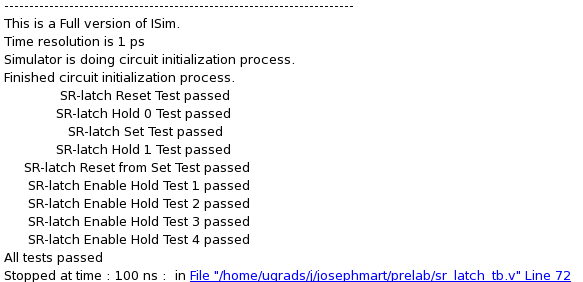
\includegraphics[scale=0.7]{sr_latch_tests.png}
      \caption{\textit{SR Latch Test Results}}
    \end{center}
  \end{figure}
  \newpage
  \begin{figure}[h]
    \begin{center}
      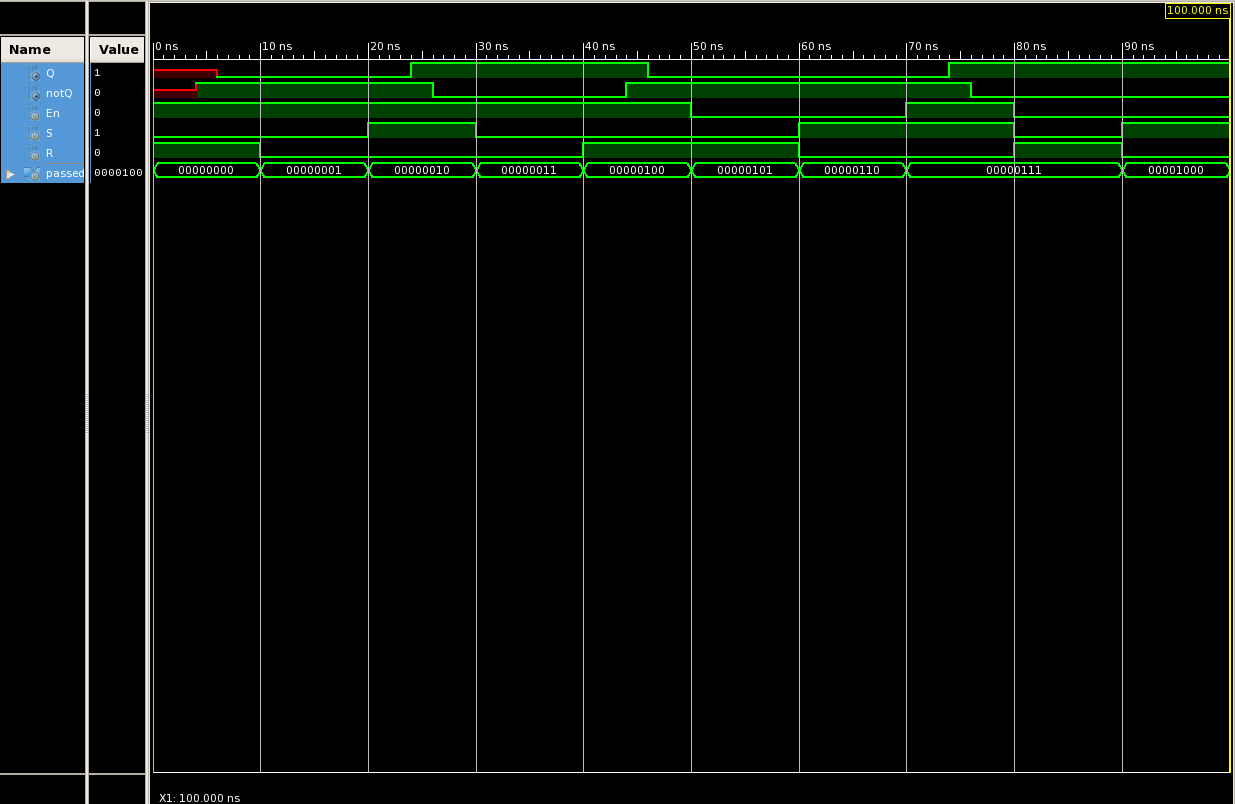
\includegraphics[scale=0.3]{sr_latch_graph.png}
      \caption{\textit{SR Latch Graph}}
    \end{center}
  \end{figure}
  
  The next test was again for the SR-Latch but this time, the gates had a four
  second delay instead of two. The test results are below.
  
  \begin{figure}[h]
    \begin{center}
      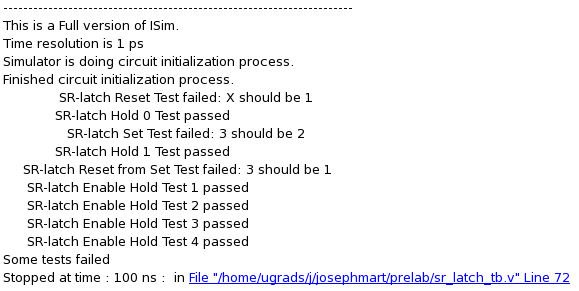
\includegraphics[scale=0.53]{sr_latch2_tests.png}
      \caption{\textit{SR Latch2 Test Results}}
    \end{center}
  \end{figure}
  
  \newpage
  
  \begin{figure}[h]
    \begin{center}
      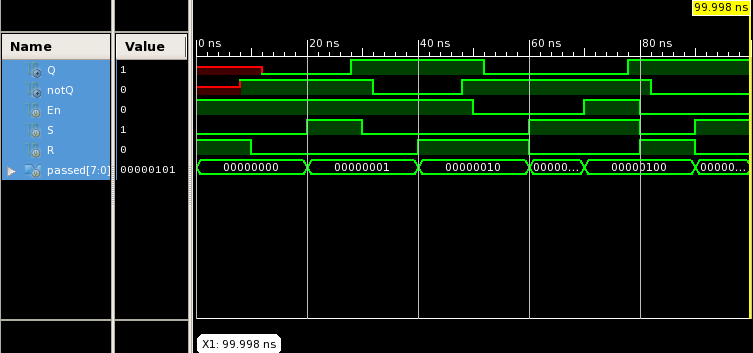
\includegraphics[scale=0.4]{sr_latch2_graph.png}
      \caption{\textit{SR Latch2 Graph}}
    \end{center}
  \end{figure}
  
  The test for the four nanosecond delay failed the first four reset
  , hold, and set tests. For instances where the four delay was in line
  with the two delay, the test passed
  
  Next, the D-Latch was tested against the provided test bench. The operation
  matched the given table in the lab. The test results are below.
  
  \begin{figure}[h]
    \begin{center}
      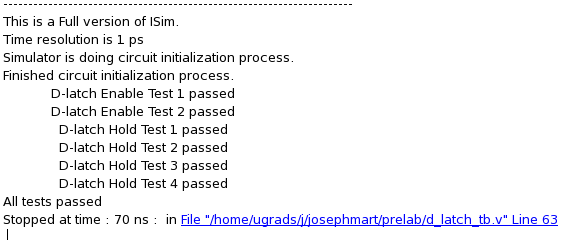
\includegraphics[scale=0.7]{D_latch_tests.png}
      \caption{\textit{D-Latch Test Results}}
    \end{center}
  \end{figure}  
  
  \newpage
  
  \begin{figure}[h]
    \begin{center}
      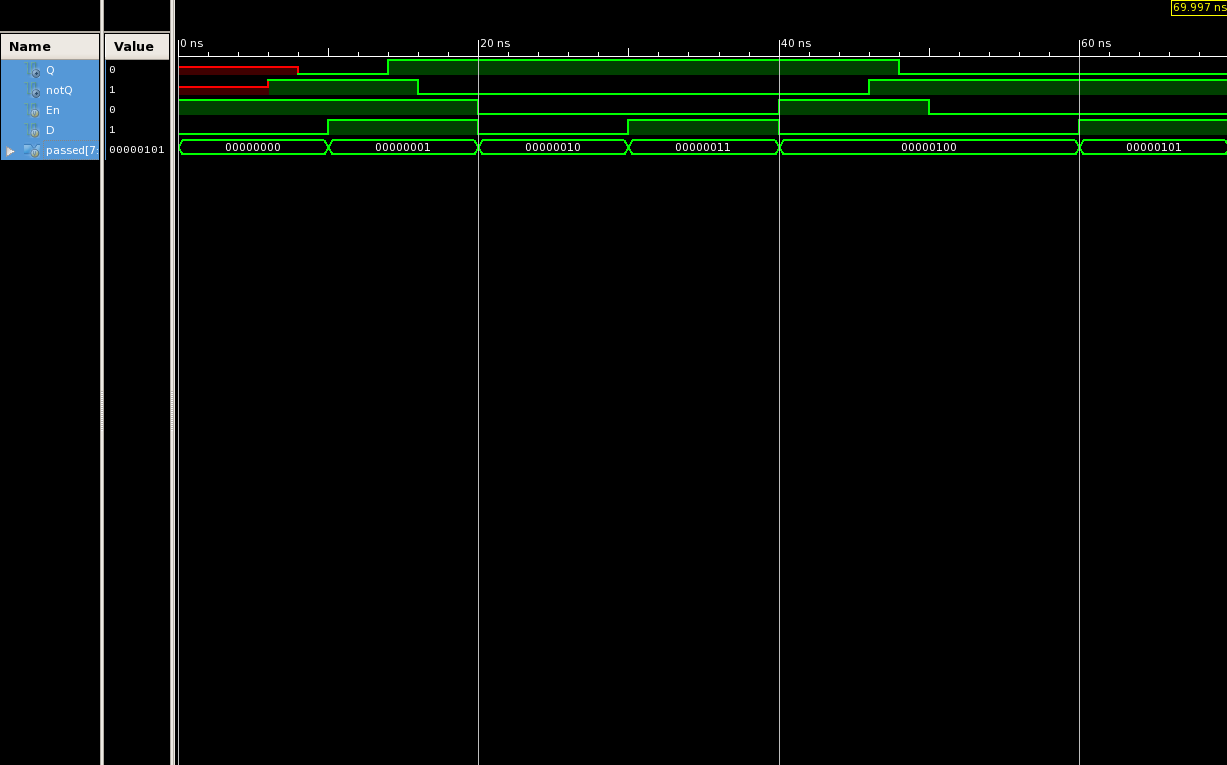
\includegraphics[scale=0.2]{D_latch_graph.png}
      \caption{\textit{D-Latch Graph}}
    \end{center}
  \end{figure}
  
  The D flip-flop was then tested against the appropriate test bench
  with internal nets in the waveform.
  
  \begin{figure}[h]
    \begin{center}
      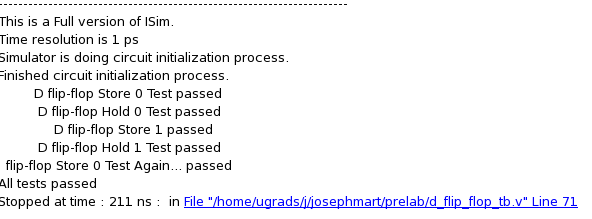
\includegraphics[scale=0.7]{Master_Slave_D_flip_flop_tests.png}
      \caption{\textit{D Flip-Flop Tests}}
    \end{center}
  \end{figure}
  
  \newpage
  
  \begin{figure}[h]
    \begin{center}
      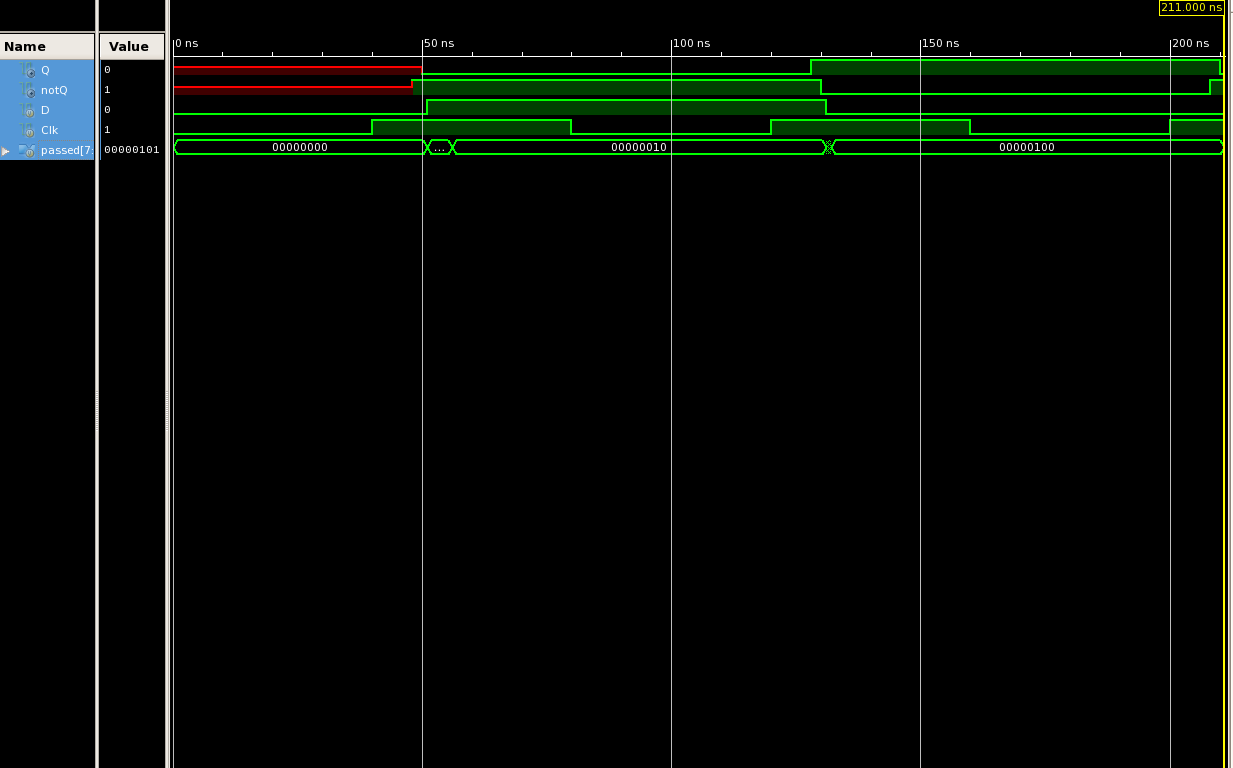
\includegraphics[scale=0.32]{Master_Slave_D_flip_flop_graph.png}
      \caption{\textit{D Flip-Flop Graph}}
    \end{center}
  \end{figure}
  
  The internal nets behaved as expected.
  
  In the final part of \textbf{Experiment 1}, the behavioral D-Latch and
  D flip-flop was tested against their appropriate test benches.

  \begin{figure}[h]
    \begin{center}
      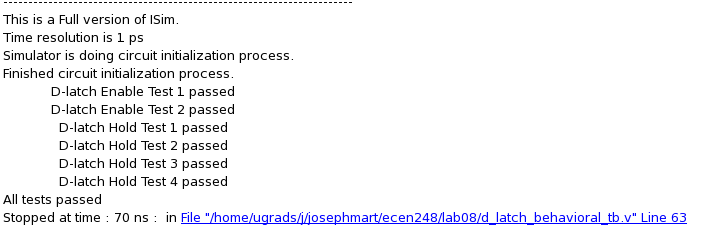
\includegraphics[scale=0.6]{d_latch_Behavioral_tests.png}
      \caption{\textit{D Latch Behavioral Test Results}}
    \end{center}
  \end{figure}
  
  \newpage
  
  \begin{figure}[h]
    \begin{center}
      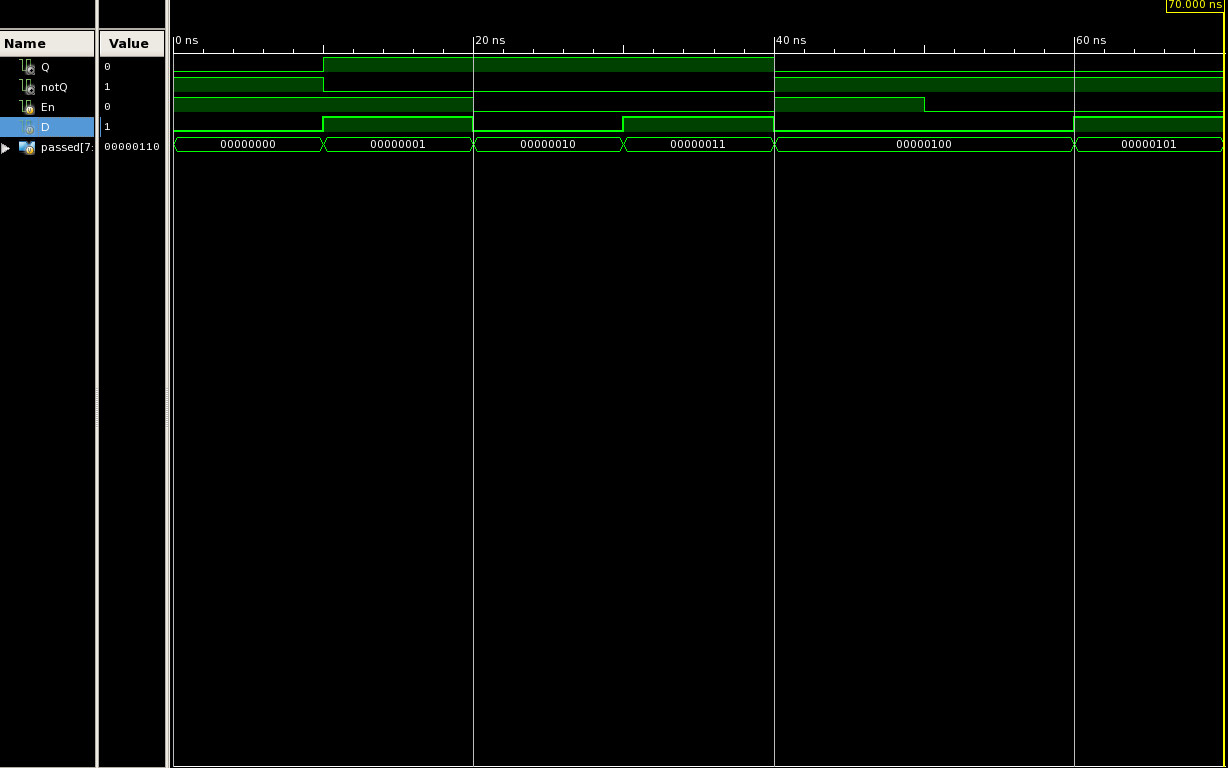
\includegraphics[scale=0.3]{d_latch_Behavioral_graph.png}
      \caption{\textit{D Latch Behavioral Graph}}
    \end{center}
  \end{figure}

  \begin{figure}[h]
    \begin{center}
      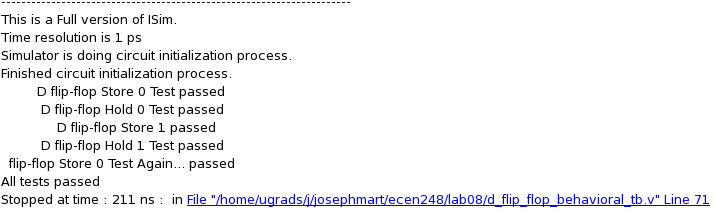
\includegraphics[scale=0.55]{d_flipflip_behavioral_tests.png}
      \caption{\textit{D Flip Flop Behavioral Test Results}}
    \end{center}
  \end{figure}
  
  \newpage
  
  \begin{figure}[h]
    \begin{center}
      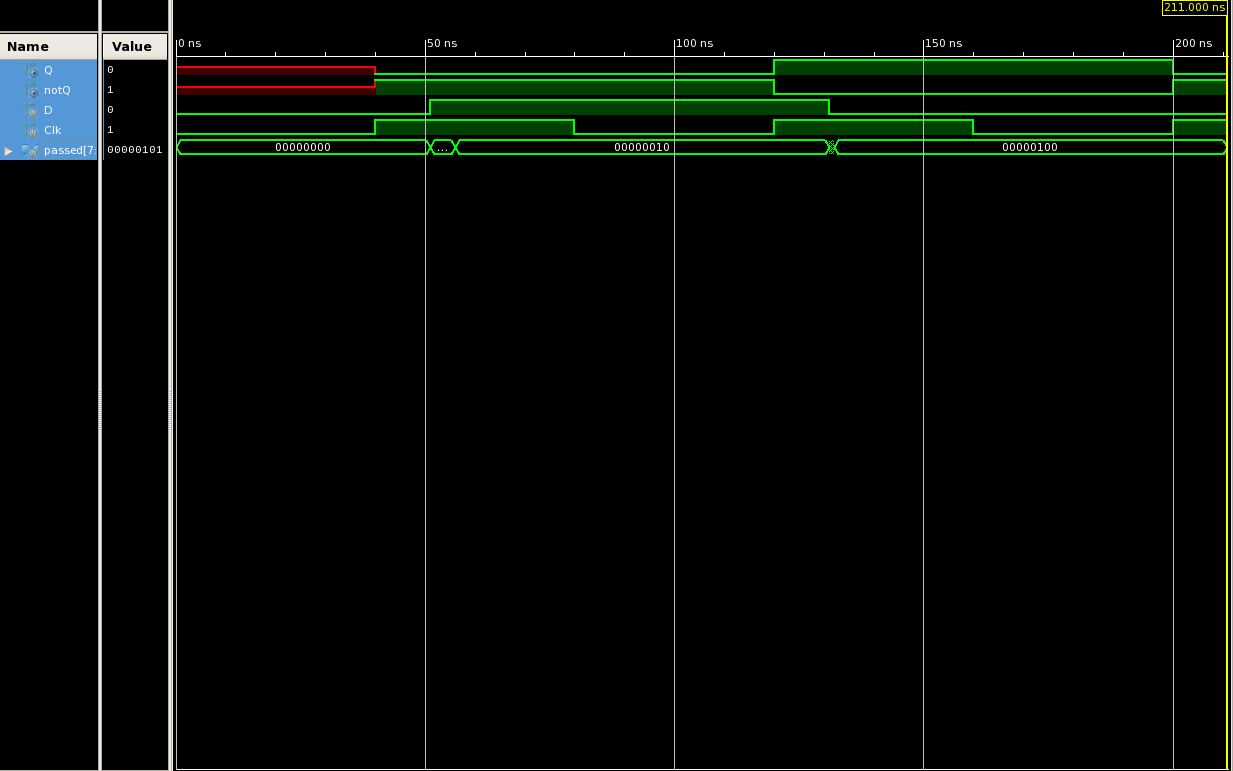
\includegraphics[scale=0.35]{d_flipflip_behavioral_graph.png}
      \caption{\textit{D Flip Flop Behavioral Graph}}
    \end{center}
  \end{figure}
  
  The behavioral and structual D flip-flop design looked identical. The
  structual and behavioral D-latch differed for the first eight nanoseconds
  where Q and notQ were switched.
  
  \textbf{Experiment 2}
  
  In \textbf{Experiment 2}, the 2-Bit adder was tested against my written
  test bench. It passed all test vectors.
  
  \begin{figure}[h]
    \begin{center}
      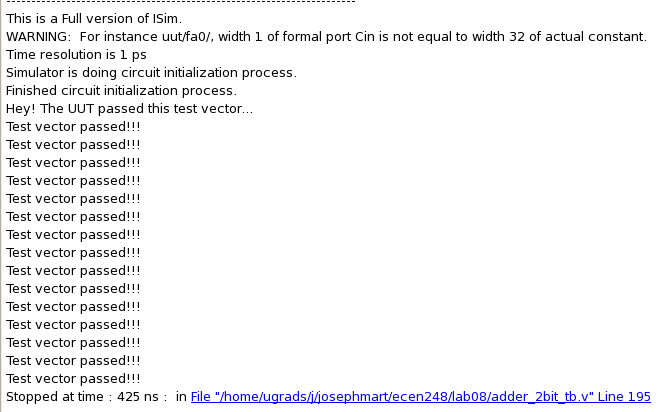
\includegraphics[scale=0.3]{adder2bit_tests.png}
      \caption{\textit{2-bit Adder Test Results}}
    \end{center}
  \end{figure}
  
  \newpage
  
  \begin{figure}[h]
    \begin{center}
      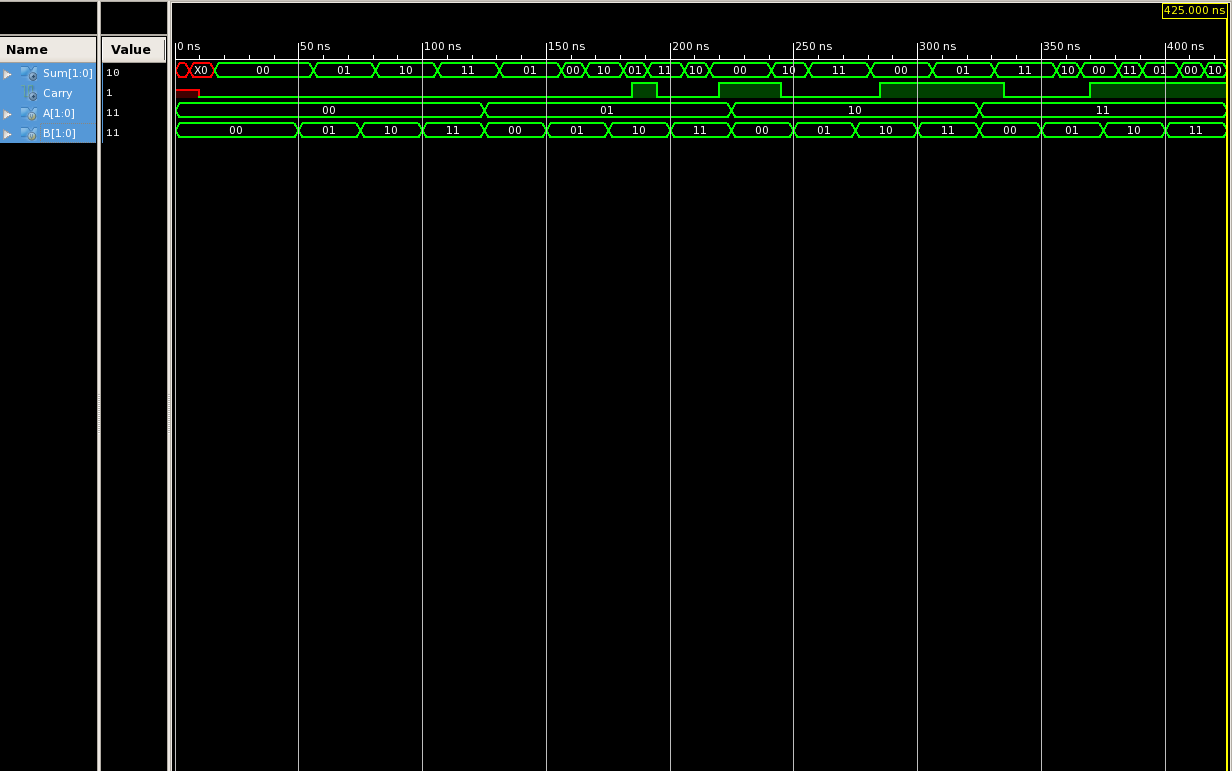
\includegraphics[scale=0.2]{adder2bit_graph.png}
      \caption{\textit{2-Bit Adder Graph}}
    \end{center}
  \end{figure}
  
  Finally, the synchronous adder circuit was tested against the test bench
  ‘define CLOCK PERIOD being set to 40. Then with 18, 19, and 20. 40, 18,
  and 20 are shown below.
  
  \begin{figure}[h]
    \begin{center}
      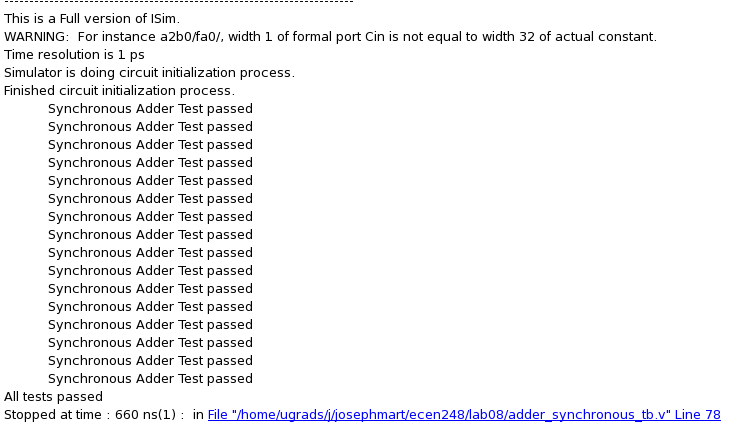
\includegraphics[scale=0.5]{asyc40_tests.png}
      \caption{\textit{Asyc 40 Tests}}
    \end{center}
  \end{figure}
  
  \newpage

  \begin{figure}[h]
    \begin{center}
      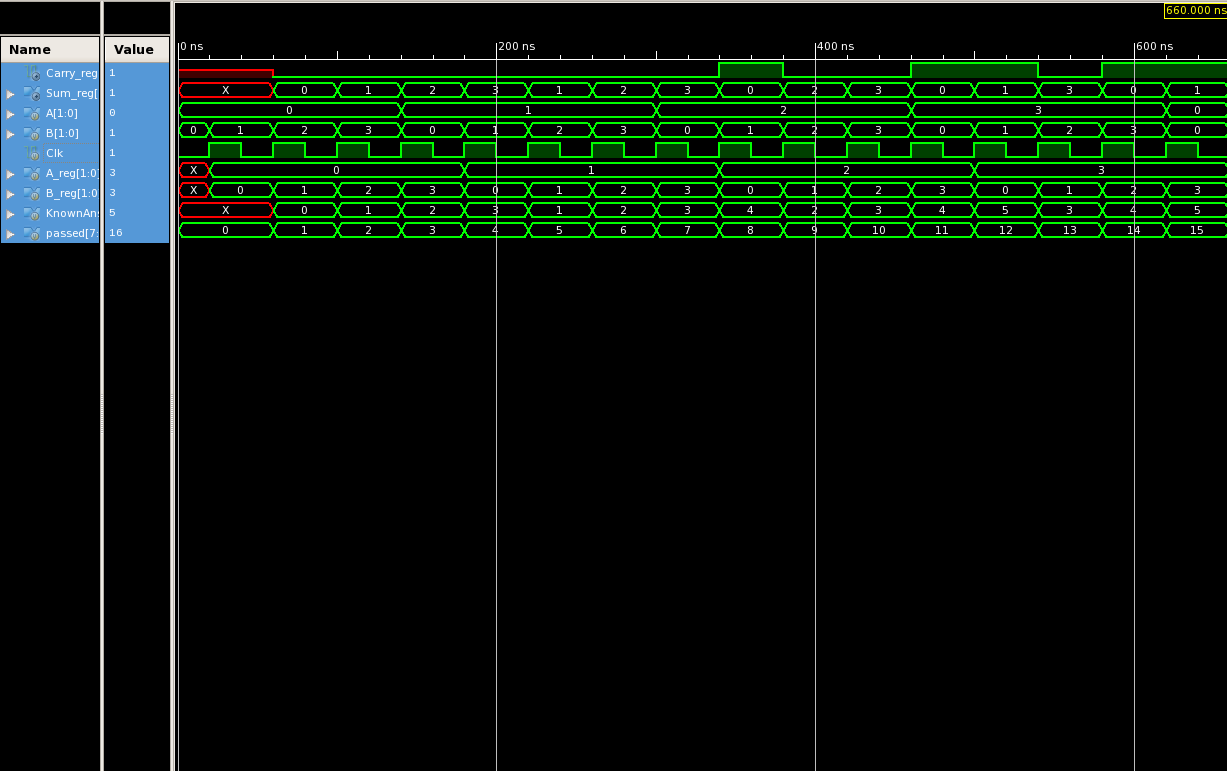
\includegraphics[scale=0.3]{asyc40_graph.png}
      \caption{\textit{Asyc 40 Graph}}
    \end{center}
  \end{figure}
  
  \begin{figure}[h]
    \begin{center}
      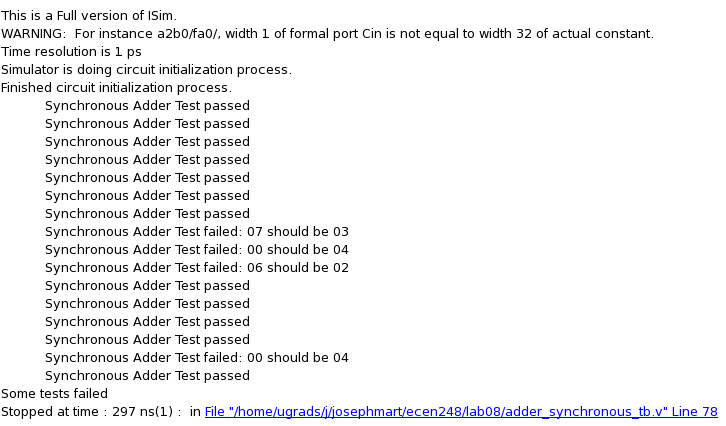
\includegraphics[scale=0.35]{asyc_18_tests.png}
      \caption{\textit{Asyc 18 Tests}}
    \end{center}
  \end{figure}
  
  \newpage
  
  \begin{figure}[h]
    \begin{center}
      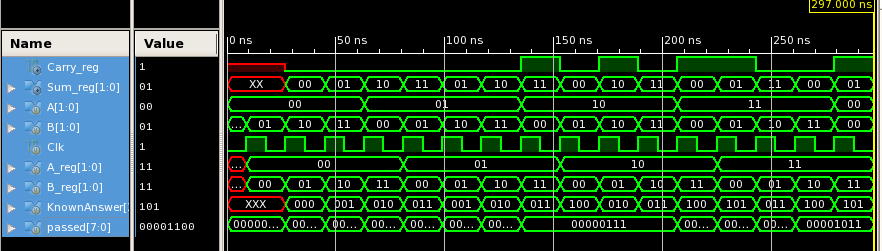
\includegraphics[scale=0.4]{asyc_18_graph.png}
      \caption{\textit{Asyc 18 Graph}}
    \end{center}
  \end{figure}
  
  \begin{figure}[h]
    \begin{center}
      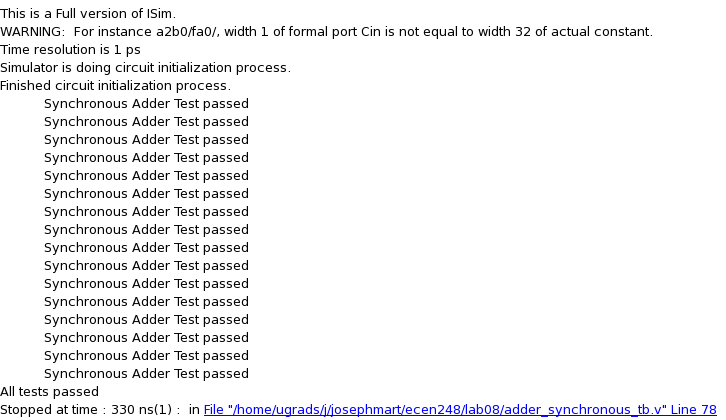
\includegraphics[scale=0.5]{asyc_20_tests.png}
      \caption{\textit{Asyc 20 Tests}}
    \end{center}
  \end{figure}
  
  \newpage
  
  \begin{figure}[h]
    \begin{center}
      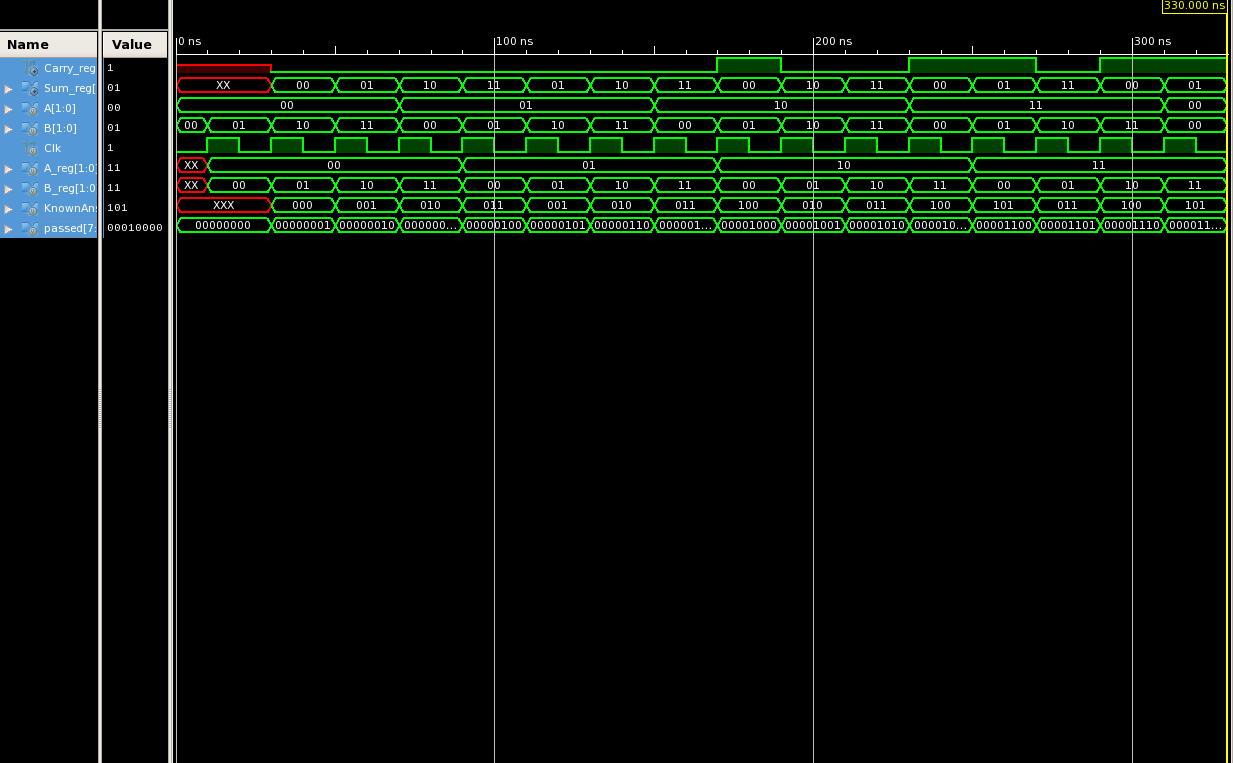
\includegraphics[scale=0.3]{asyc_20_graph.png}
      \caption{\textit{Asyc 20 Graph}}
    \end{center}
  \end{figure}
  
  The test passed for 40 and 20 and failed for 18 and 19. Thus the shorest
  $`define CLOCK PERIOD = 20ns$
  
\section*{Conclution}

  \hspace{15pt}In conclution, this lab exposed me to test bench code by
  allowing me to create my own for the first time. Also, this lab introduced
  me to three different type of latches, SR latch, D latch, and D flip-flop latch.

\section*{Questions}

\begin{enumerate}
  \item \textbf{Include the source code with comments for all modules you
    simulated. You do not have to include test bench code that was
    provided; however, you must supply the test bench code that you wrote! Code
    without comments will not be accepted.}

    \textit{In the report.}

  \item \textbf{Include screenshots of all waveforms captured during simulatio in addition
    to the test bench console output for each test bench simulation.}

    \textit{In the report.}

  \item \textbf{Answer \underline{all} questions throughout the lab manual.}

    \textit{In the report.}

  \item \textbf{Compare the behavioral description of the synchronous adder found in the
    test bench code with the combination of stuctual and dataflow Verilog you
    used in the lab assignment. What are the advantages and disadvantages of each?
    Which do you perfer and why?}
    
    The advantage of utilizing a behavioral description is that it is very simple and to the point because
    it uses one statement that then decides what kind of output it is going to be. In structural and dataflow
    Verilog it is precise, but not all that concise. Efficiency is lost because it must look for each specific
    output rather than just paying attention to the output behavior as a whole. I prefer behavioral Verilog
    because it seems like it is a whole lot more efficient. 

  \item \textbf{Based on the clock period you measured for your synchronous adder, what
    would be the theoretical maximum clock rate? What would be the effect of
    increasing the width of the adder on the clock rate? How might you improve the
    clock rate of the design?}
    
    The smallest `define CLOCK PERIOD that the circuit could of been reduced to and still function
    was 20 ns which works at a 50MHz clock rate. Increasing the width of the adder would cause the
    clock rate to drop because it has to work with more inputs. This would result in a greater time
    delay which would result in a drop in clock rate. Improving the clock rate of the design would
    be done by decreasing the time delay in the circuit by simplifying the circuit have to use less
    or by using gates that have a smaller gate delay.

\end{enumerate}

\section*{Student Feedback}

\begin{enumerate}
  \item \textbf{What did you like most about the lab assignment and why? What did you like least aboub it and why?}

  I enoyed learning about test bench workings. I also liked practicing more with Verilog.

  \item \textbf{Were there any section of the lab manual that were unclear? If so, what was unclear? Do you have any suggetions for improving the clarity?}

  This lab was very straight forward and provided more guidance than most of the previose labs.

  \item \textbf{What suggestions do you have to improve the overall lab assignment?}

  Synthesising the designs onto the Spartan board would of been cool.

\end{enumerate}

\ifx
\begin{thebibliography}{1}
\bibitem{Verilog} Charles Kime \& Thomas Kaminski  \emph{Logic and Computer Design Fundamentals} \\ \hspace{15pt}\textit{http://www.cs.bilkent.edu.tr/~will/courses/CS223/Verilog/LCDF3_Verilog_Ch_4.pdf}
\end{thebibliography}

\section*{Attachments}
%Make sure to change these
Lab Notes, HelloWorld.ic, FooBar.ic
%\fi %comment me out

\begin{thebibliography}{9}
\bibitem{Verilog} Charles Kime & Thomas Kaminski  \emph{Logic and Computer Design Fundamentals} \textit{http://www.cs.bilkent.edu.tr/~will/courses/CS223/Verilog/LCDF3_Verilog_Ch_4.pdf}
\end{thebibliography}

%How to cite
Put your Problem statement here! Example of a Citation\cite[p.219]{Robotics}. Here's Another Citation\cite{Flueck}
\fi
\end{document}
